\documentclass[a4paper,10pt]{article}
\usepackage{isolatin1}
\usepackage{graphicx}
%\usepackage[dvips]{graphicx}
%\usepackage{epsfig}
\usepackage{rotating}
\usepackage{subfigure}
\usepackage{mlverb}

\usepackage{a4wide}
\usepackage{array}
\usepackage{lastpage}
\usepackage{url}

\usepackage[numbers,sort]{natbib}
%\usepackage{natbib}
\bibliographystyle{plainnat}
%\bibliographystyle{abbrvnat}
%\bibliographystyle{unsrtnat}

%\bibliographystyle{plain}

\addtolength{\headheight}{3pt}

%rm pis.ps && latex report.tex && latex report.tex && dvips -o report.ps report.dvi && psselect -p1-26 report.ps > pis.ps && a2ps --border=no -1 -oprint.ps pis.ps appendixA.ps appendixB.ps appendixC.ps appendixD.ps appendixE.ps appendixF.ps appendixG.ps appendixH.ps

\newcommand{\floatfigure}[4]{ %filnavn, bredde/hoejde, caption, label
%  \begin{figure}[htbp]
  \begin{figure}[ptb]
    \begin{center}
      \leavevmode %Apparently an old trick to fix a bug related to center...
      \includegraphics[#2]{#1}        
      \caption{#3}
      \label{#4}
    \end{center}
  \end{figure}
}

\makeatletter
% Make the caption italic
\renewcommand{\fnum@figure}[1]{\textbf{\figurename~\thefigure} --
  \itshape}
\renewcommand{\fnum@table}[1]{\textbf{\tablename~\thetable} --
  \itshape}
\makeatother

\begin{document}
\section*{Introduction}
This document briefly describes the design of TinyBT (section
\ref{tinybt}) and introduces how to write applications using it
(section \ref{progtbt}).

For further information on TinyBT and experiments using TinyBT see
\cite{leo03bluetooth}.

\section{TinyBT Design}
\label{tinybt}
The first goal of this stack not compatibility to connect to all
Bluetooth devices, but rather feasibility in a sensor network.
Therefore we took a minimalistic ``bottom-up'' approach implementing
features from the specification: we will design example applications
and only implement the features that are required for these
applications and thus keeping the features of the stack at a bare
minimum. The implemented application is the benchmarking program for
our experiments (see section \ref{experiments}) and a self-assembly
routing network.

Today a number of open source Bluetooth host stacks exists that can
serve as inspiration when building TinyBT. Affix and Bluez are the two
leading implementations for Linux and the Smart ITs team has developed
an simple embedded operating system and Bluetooth stack specifically
for the BTNode. All of which have served as inspiration while
developing TinyBT. For more information on Bluez see \cite{ML02}.

\subsection{TinyBT Components}
The Bluetooth specification distinguishes the ``Bluetooth host'' from
the ``host controller'' (Bluetooth hardware) - see figure
\ref{fig:btcomponent}. The host implements the upper layers of
Bluetooth (l2cap, sdp, profiles) and the lower layers (lm, bb) are
embedded in the host controller. The interface between the two is
denoted Host Control Interface (HCI). We split the design into
software components that resemble the logical abstractions of the
Bluetooth specification:

\begin{description}
\item [Physical Bus Driver] abstracting the characteristics of the
  physical bus; on the BTnodes the UART connecting the MCU and the
  Bluetooth radio. We implement this as the component \emph{HCIPacket}
  - figure \ref{fig:tinybtimplem}, see section \ref{hcipacket}.
\item [HCI Driver] This layer maps the interface of the underlying HCI
  layer (the upper layer embedded on the Bluetooth radio) into the
  programming model used for implementing the higher layers. We
  implement this as the component \emph{HCICore} - figure
  \ref{fig:tinybtimplem}, see section \ref{hcicore}.
\end{description}

\begin{figure}[tbp]
\centering
\subfigure[Bluetooth]{
  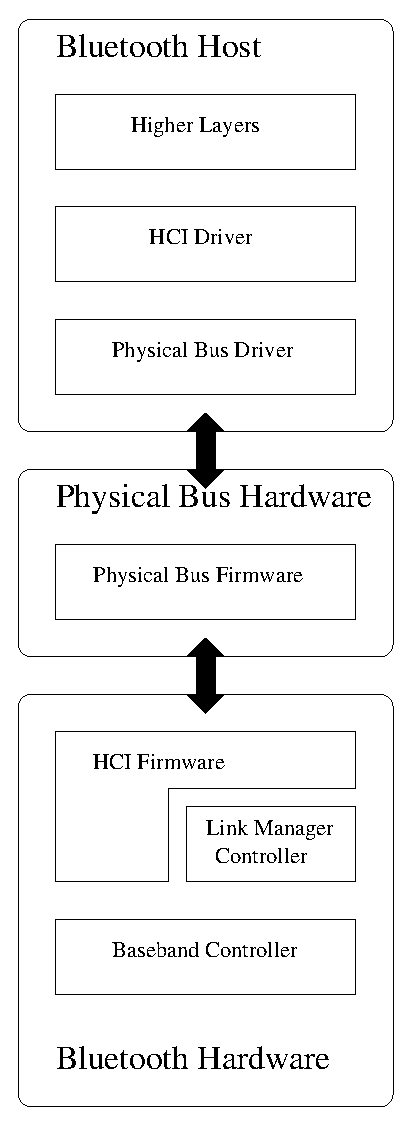
\includegraphics[height=0.35\textwidth]{hci}
  \label{fig:btcomponent}
}
\subfigure[TinyBT component model]{
  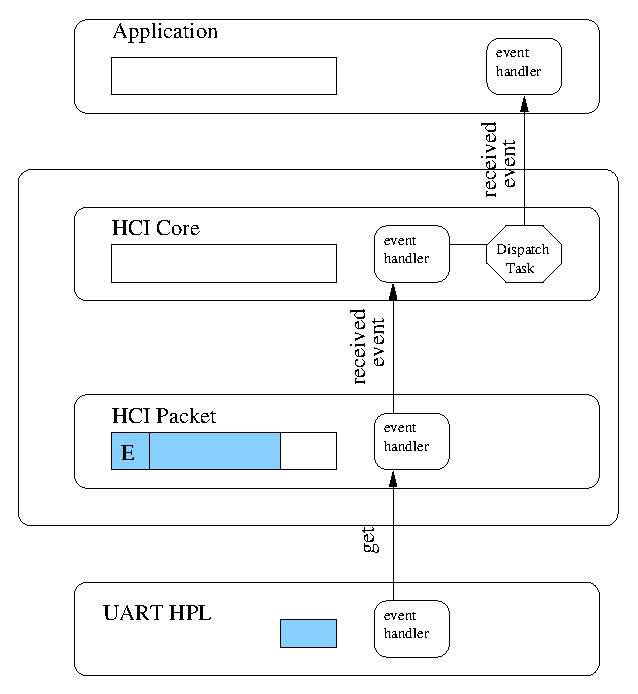
\includegraphics[width=0.35\textwidth]{implem}
  \label{fig:tinybtimplem}
}
%\subfigure[TinyBT component model]{
%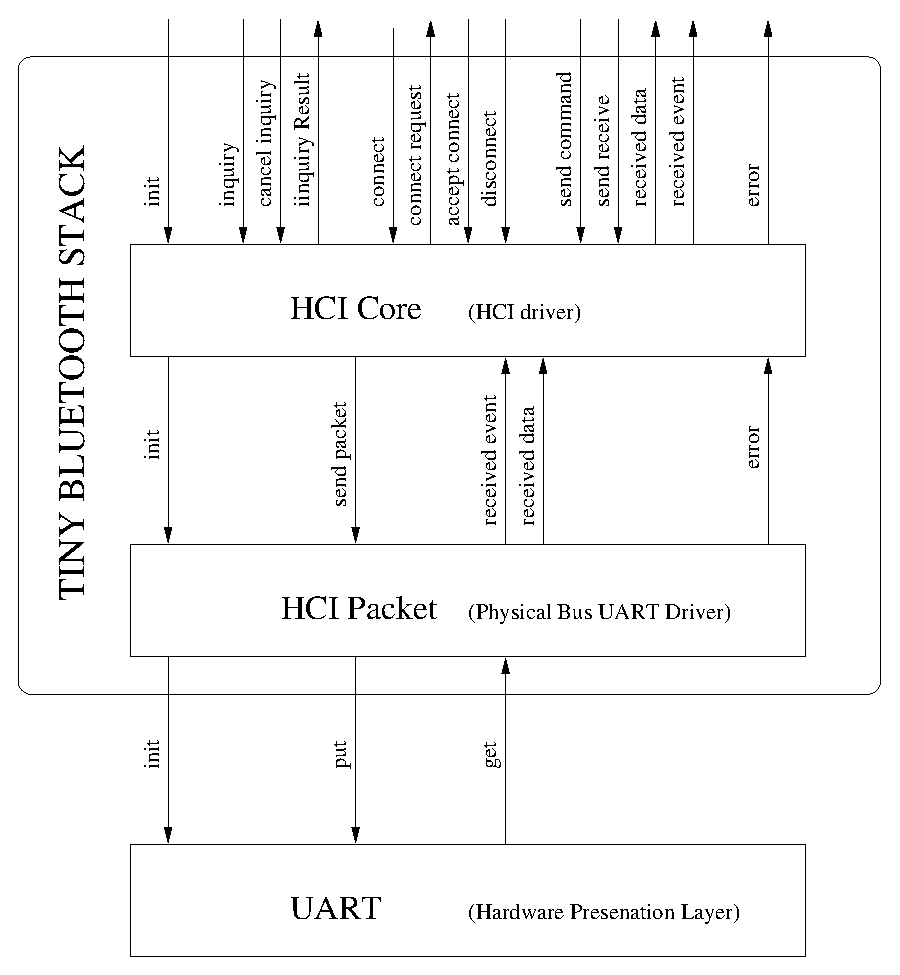
\includegraphics[width=0.35\textwidth]{tinybluetooth}
%\label{fig:tinybtcomponent}
\caption{Abstract software layer model from the Bluetooth
  specification and the component model of the TinyBT stack. Buffers
  are show as boxes inside each component.}
\end{figure}

\subsubsection{Events}
The path of the events through the system is shown in figure
\ref{fig:tinybtimplem}. The UART signals HCIPacket for each byte
received over the air. From these bytes HCIPacket constructs an entire
HCI-packet (in the form of a \emph{gen\_pkt} - section
\ref{bufferstructure}) as soon as an entire packet has been assembled
it signals HCICore. HCICore dispatches a task that parses the event
and signals the application.

In the figure the number of standby-buffers is shown. The UART has a
buffer ready for each incoming byte. HCICore has a buffer to construct
entire packets. It is unlikely that HCICore is able to handle an event
so fast the a new buffer is not required to store bytes from the uart
while HCICore processes the event. For this reason HCICore has a
buffer standing by that it trades with the one from the lower layers.
The application can have any number of buffers standing by as
required.

\subsubsection{Error handling}
The TinyBT system has a large number of places that errors could
occur; synchronization with the UART, packet loss and many more.
Handling errors in a convenient manor is a requirement. In TinyOS we
lack operating system features such as exceptions or assertions that
would aid us in taking appropriate action upon error conditions. Our
solution is to extend each component with an error event that is
signaled with commonly defined error codes. HCIPacket signals HCICore
which in turn signals the application that is able to perform desired
error recovery or abort - see figure \ref{fig:tinybtcomponent}.

\subsubsection{UART handling}
The original TinyOS UART component was not designed with high
throughput in mind and it was not used at high speeds in the original
stack. As such we observed that we were not able to drive the
throughput to more than app. 35 $\frac{kB}{s}$.

The UART transmits bit serially using two registers: a shift register
that shifts bits of the current byte over the serial line and a buffer
register that holds the next byte to be sent. The UART can signal that
it is ready to receive more data in two ways: Either when the shift
register is empty and there is no more bits to send (TXCIE) or when
the next byte to be sent moves from the buffer register to the shift
register (UDRIE). The TinyOS implementation was based on the TXCIE
interrupt --- this has the unfortunate consequence that the UART has
to wait until the MCU has started the interrupt handler and it has
located the next byte to send. This latency is likely to cause timing
problems and a drop in performance.

We measured the actual UART speed using 3 modes of transmission:
either \mbox{TXCIE}/\mbox{UDRIE} interrupts or polled transmission. The
results in table \ref{tab:uart} show that using UDRIE is able to give
as good performance as polled transmission and that they are both able
to fill the bandwidth of the serial line\footnote{Serial encoding 8n1 (8
data bits, no parity, 1 stop bit, 1 start) means that 20\% of the line
capacity is wasted}.

\begin{table}[tbp]
  \begin{center}
    \begin{tabular}{|c|c|c|c|c|c|c|}
      \hline
      Rate & \multicolumn{2}{c|}{Ideal} & 8N1 & TXCIE & UDRIE & polled\\
      $\frac{kb}{s}$ & $\frac{kB}{s}$ & $\frac{KiB}{s}$ &$\frac{kB}{s}$ &$\frac{kB}{s}$  &$\frac{kB}{s}$ &$\frac{kB}{s}$ \\
      \hline
      460.8 &  57.60  & 56.25 & 46.08 &  35.21 &   46.08 &  46.08\\
      \hline
    \end{tabular}
    \caption{Measured UART rates when communicating in 3 different
      ways: using either \mbox{TXCIE}/UDRIE interrupts or polled
      transmission.  Lower case ``k'' refers to 1000, ``Ki'' refers to
      1024, ``b'' to bits, ``B'' to bytes. The UART uses 8N1 encoding
      resulting in only an 80\% effective throughput of the bits sent
      on the serial line.}
    \label{tab:uart}
  \end{center}
\end{table}

\subsection{Buffer structure}
\label{bufferstructure}
In order to be able to take advantage of the ``buffer trading'' style
of memory management, we design a data structure that will be used
throughout the Bluetooth subsystem. Since it is fixed and well defined
we can trade any one instance for any other. In this way no layer needs
to copy any part of the package before handing it off to an other
module. Of course this has the disadvantage that the buffer is
required to be ``big enough''.

We let our selves be inspired by Linux socket buffers \cite{TLK} and
use an interface that resemble slightly to pass packets from module to
module: \emph{gen\_pkt} (figure \ref{fig:buffer}). This is done using
a simple data structure, that besides a chunk of data it has a
\emph{start} and \emph{end} pointer that allow for easy header
removal/insertion. A sending application start filling in bytes from
the end of the data chunk and receiving applications start at the
beginning and move the start pointer when a header is added or
removed.

An other design choice could have been to add headers as a linked list
instead (as for example the FreeBSD \emph{mbufs} structure
\cite{LMKQ90}), however having a buffer of a non-fixed size would
complicate the trading procedure.

To increase the readability of the program and be able to use the help
that the type checking system can give at compile time, the
\emph{gen\_pkt} is type cast into a number of specific buffer types,
that are specific to a certain command or event.  This allows passing
buffers between modules without copying from general to specific
structures while still taking advantage of the type system. For
example the packet \emph{sniff\_mode\_pkt} (figure \ref{fig:buffer})
is the packet used to turn the ``sniff-mode'' feature on or off: it
has a field called \emph{cp} of the type \emph{sniff\_mode\_cp} that
contains all the arguments required to negotiate sniff mode such that
the programmer need not worry about the exact bit-order etc.

\begin{figure}[tbp]
  \centering
\begin{scriptsize}
\begin{tabular}{ll}
\verb+ typedef struct {+  &          \verb+ typedef struct {+ \\
\verb+     uint8_t *end;+         & \verb+     uint8_t *end;+\\
\verb+     uint8_t *start;+       & \verb+     sniff_mode_cp *start;+\\
\verb+     uint8_t data[HCIPACKET_BUF_SIZE];+ & 
\verb+     uint8_t data[HCIPACKET_BUFSIZE-sizeof(sniff_mode_cp)];+\\
\verb+ } __attribute__ ((packed)) gen_packet;+ &  \verb+     sniff_mode_cp cp;+ \\
                     &    \verb+ } __attribute__ ((packed)) sniff_mode_pkt;+ 
\end{tabular}
\end{scriptsize}
  \caption{Generic (left) and specific bufferstructure (right).}
  \label{fig:buffer}
\end{figure}

We still need to calculate the required size of the buffer in advance
to make sure that when each layer adds headers by moving the ``start''
pointer we will not exceed the boundary of the buffer. In TinyBT this
is handled by defining two constants ``HCIPACKET\_BUF\_SIZE'' and
``MAX\_DLEN'' describing the buffer size and the maximum packet payload
size that leaves room for all header in the stack. The maximum data
length (dlen) and number of buffers that the host controller is able
to store should be communicated to the Bluetooth module using the
command ``Host\_Buffer\_Size''\cite{BT02, 4.7.41} however this has not
been implemented in TinyBT at the time of writing. If the data length
of the transmitter is no larger than that of the receiver this will
not result in problems, but could in general result in eronous
behavior.

An interesting solution to this problem is presented in \cite{Ye02b}.
In order to derivate the correct size of all headers in the system
with as little effort as possible each layer \emph{embeds} the headers
of lower layers in its own such that the header structure for layer n
contains the headers for all layers $<$ n. It would be easy to apply
this approach to our design and would allow the compiler calculate
buffer space required to contain all headers.

\subsection{HCIPacket}
\label{hcipacket}

\begin{figure}[ptb]
  \begin{center}
    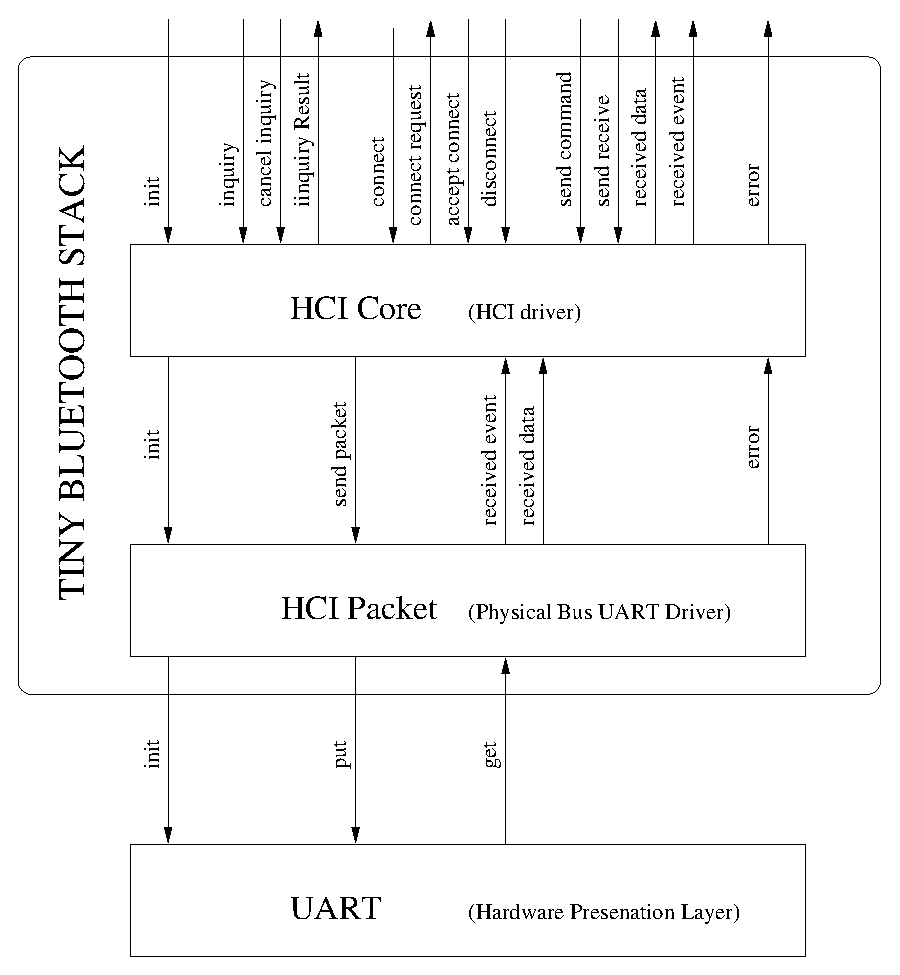
\includegraphics[width=0.35\textwidth]{tinybluetooth} 
    \caption{Event path in TinyBT}
    \label{fig:tinybtcomponent}
  \end{center}
\end{figure}

The HCIPacket component provides a packet based interface to the
Bluetooth hardware. It signals upper layers upon receiving entire HCI
packets and is thus independent of the underlying hardware, this could
be packet based such as USB, byte-based as in our case or even a
simulator if required (see section \ref{simulation}).

The interface for HCIPacket shown in figure \ref{fig:tinybtcomponent}
between the HCIPacket and HCICore components exports only a few command
and events: initialisation and error handling, packet transmission,
event reception and data reception. 

Event and data reception is handled as one event each to match the
fact that Bluetooth considers each to be separate and sends them in
different packet formats. Events have to be parsed, some are for
maintenance purposes and some are for the application, data packets are
always meant for the application.

The send operation \emph{putPacket} is asynchronous as it will transmit
the packet to the Bluetooth device and signal \emph{putPacketDone}
once the buffer has been transmitted over the bus to the Bluetooth
device. During this time the buffer is owned by the HCIPacket
(ownership transfer see section \ref{bufferstructureo}). After
transmission over the serial line (or failure of the same) the buffer
is given back when the send is acknowledged with a
\emph{putPacketDone} signal.

\subsection{HCICore}
\label{hcicore}
The HCI interface mentioned previously enables a Bluetooth host
controller to communicates with its host via a command/events
semantics. TinyOS modules communicate using a similar command/event
based system. Following this thought it would be natural to
\emph{translate} Bluetooth events to TinyOS events and TinyOS commands
to Bluetooth commands. In order to do this we define an interface
called \emph{Bluetooth} which export a TinyOS command for every
supported Bluetooth command and signals suitable events for every
Bluetooth event supported. A selection of the operations supported by
the Bluetooth interface is show in figure \ref{fig:tinybtcomponent}
not shown in the figure is a number of operations relating

Our design will be centered around a big \emph{switch/case} sentence
signalling the appropriate TinyOS events by the appropriate Bluetooth
event number. Such a construction is required either in the
application or in the Bluetooth subsystem in order to parse the data
from the Bluetooth Host Controller. Whether this parsing is done most
efficiently in the Bluetooth subsystem or the application is not going
to be explored in this report. In this design we choose to parse the
packets in the HCI layer and pass packets with appropriate events.
This simplifies application development as each application does not
require a parser.

A Bluetooth host controller has a number of buffers on board during
initialization of the module the host is required to record the size
and number of buffers. HCICore uses this information to make sure that
the Bluetooth module never runs out of packets to send - this will
increase performance. Thus a send operation will only fail once the
Bluetooth device has filled all of it's buffers.

\subsubsection{Space efficiency}
It is not clear whether this programming style will generate the most
space efficient programs.  The NesC compiler is able to detect unused
commands as ``dead'' and remove them from the generated code they are
not used in a given application. However the compiler cannot analyse
which events handlers will be called - these events are cascaded as
external events from the host controller. Thus the compiler cannot
remove the code for events that will never be called.  In most cases
there is a one-to-one mapping of which events will be returned from
which commands, so it would be possible to predict which events would
never be called. However the per-event code overhead is only in the
order of a few lines and the savings are minimal.

One could imagine several ways of resolving this. It is possible that
the NesC compiler could be extended in such a way that would be able
to foresee that some events are part of a command/event pair - for
example via hinting (or even more simple using the C preprocessor and
the \emph{DEFINE} macro). An other option would be to
split the Bluetooth interface into more interfaces requiring the
programmer to select the necessary ones and giving the compiler the
ability to remove code belonging to unused interfaces.

\subsection{Further enhancements}
While this section has detailed the design requirements and choices
made for the current implementation of TinyBT work is already
proceeding in a number of areas.

\subsubsection{L2CAP}
In some cases it will be desirable to be able for example to connect a
sensor network with a PC with a different Bluetooth host stack
implementation for example as gateway node. So for certain types of
application it might be desirable to invest the extra overhead to gain
this functionality. Our design allows this to be implemented as a
further component on top of the HCICore.

The Bluetooth protocol architecture defines ``Logical Link Control and
Adaption Protocol'' (l2cap) as the data link layer in the Bluetooth
protocol architecture \cite{BT02}[p.259]. This layer is introduced on
top of HCI and has separate signalling mechanisms and connection
establishment procedures. This means that an other non trivial layer
will have to be added in order to support this protocol. Other
implementations such as Bluez, Affix or Smart-ITs use in the same
order of code print size as HCI to implement l2cap. The l2cap defines
a number of logical channels to be multiplexed over a single ACL
connection one is reserved for l2cap signaling and one for ``group
transmission''. The concept of group transmission requires only local
signalling and no negotiation (group create/destroy, add member). The
data sent to an l2cap group is permitted to be sent using
ACL-broadcast and thus does not require that connections are set up in
advance.

The large overhead of implementing l2cap connection oriented does not
seem attractive however it would seem that it would be possible to
implement connectionless communication without a big overhead.
Connection less communication is supported by many Bluetooth devices
such as PC with Bluez or Affix, and most likely Bluetooth telephones
as well.

\subsubsection{Simulation}
\label{simulation}
The holistic TinyOS framework allows easy and accurate simulation of
the functionality of an application by providing alternate
implementations of hardware specific components that can run in other
environments such as a PC. It is essential that our design allows us
to take advantage of this easily and the hardware-abstract layers
HCIPacket or Bluetooth provide such an opportunity.

This detail of this simulation depends entirely on the implementation
of the replacement components. The Berkeley team focused on
functionality simulation rather than accurate models of the radio,
packet loss, etc. It would be possible to extend this to a more
general architecture that replaces the lower, hardware dependent
components with components connected a more detailed simulation
engine.

\floatfigure{tinyBTarch}{width=0.35\textwidth}
{Simulation and execution of the TinyBT component model}{fig:tinybtarch}

In order to simulate the radio a model of the transmission is
required. The Berkeley TinyOS team uses a simple bit level radio
however all of the MAC layers are embedded in software. This
means that in the simulation all of the software components for the
real mote can be reused. In our case our radio embeds all of the MAC
layers, thus to create a simulation we need to rewrite these layers to
create an accurate simulation. As for the TinyOS case we need to
choose a interface to replace with simulated components, we have 3
interfaces in play: The UART, HCIPacket and Bluetooth. It would
not make sense to convert packets to a stream of bytes and simulate a
UART; it would make sense to simulate either HCIPacket or
Bluetooth. The job of HCICore is to parse data in the HCI-format and
signal the appropriate events in the Bluetooth interface. A simulator
of the lower levels has just simulated these events and would have to
wrap this up in an HCI-event packet and send it to the HCICore. As such the
HCICore component is unnecessary in the simulation. Therefore the
initial work started by Dennis Haney has concentrated on
simulating the Bluetooth interface, this of course precludes us from
using the simulator to test the HCICore component.

\subsubsection{Power control}
In sensor nodes such as our BTNode, power is a scarce resource and has
to be used very carefully. Controlling the power usage is thus a prime
issue.

There a number of tuning knobs to turn when optimizing the power
consumption using the BTNode (see section \ref{powersave}):
\begin{itemize}
\item Park/sniff mode: The BT module sleeps for extended periods
  allowing the ROK module to power down it's radio. On negotiated
  intervals the module wakes up to synchronize the radio. When
  entering parked state a module gives up it's ``active member
  address'' and is not as such a part of a piconet.
  
\item Turning the ROK module off either using the faulty off-signal or
  using the BTNode off-switch.
  
\item Similarly the Atmega 128 has low power operation modes that
  allows it to sleep until woken by external interrupts. TinyOS enters
  this state when it has run out of tasks to schedule (like the
  ``idle'' process of traditional operating system.

\end{itemize}

With these modes in mind, how should the decision when to power down
the ROK module be made? The MCU power down mode is possible since the
MCU can woken instantly. With the BT module however there is a certain
amount of overhead involved in either entering park-mode or power-off.

Such power control could be based on statistics such as timeouts or
more elaborate schemes however it is important to notice that
information is available at the application level that could be
leveraged to perform the most optimal power control.

A simple measure could be for example to turn off the radio if it is
unused during extended periods of time. This could be implemented
either directly in the application or as a separate service (in
HCICore for example).  Instead of waiting for the a simple timeout to
turn off the radio it would be possible to turn off the radio if the
application has knowledge that the radio will not be used for a period
of time.

\section{Programming TinyBT}
\label{progtbt}
This section describes in more detail how to write programs for the
TinyBT stack. The stack is accessible through the Bluetooth interface
and here we only describe the most commonly used commands and evens
however the usage of the remaining is very similar and should be
deductible from the described commands.

\subsection{Memory management}
All commands in the Bluetooth interface are split-phase such that the
command starts transferring the command to the Bluetooth module as
soon as the command is executed and returns a while later. During the
execution of the command the buffer-space associated with the command
(arguments) is owned by HCICore and needs to be acknowledged when it
is no longer needed. Some commands have return arguments from the
Bluetooth module while most don't. For each ``post''-command that has
return arguments there is a corresponding ``Complete'' event for
example \emph{postReadBDAddr} reads the local Bluetooth address and
returns with a \emph{readBDAddrComplete}. The ones that do not have
return parameters acknowledge buffers using the generic
\emph{postComplete} event.

As mentioned previously we don't have resources for elaborate memory
management algorithms. The simplest model is simply to have only a
single \emph{gen\_pkt} buffer that is used to talk with HCICore.
However for some applications this might not be enough. In our example
programs we define \emph{get\_buf} and \emph{free\_buf} which simply
maintains a list of empty buffers.

All commands that return \emph{result\_t} have in common that if a
FAIL is returned no corresponding \emph{postComplete} is generated ---
this is important in the case some form of get/free is used like
above: upon FAIL the packet must be freed somewhere else than the
event handler of \emph{postComplete}.

\subsection{Initialization}
The Bluetooth module has to be initialized before it can be used. This
requires some negotiation with the Bluetooth device for which a buffer
is required. The buffer will be returned in a \emph{postComplete}
event later.

\begin{boxedverbatim}
command result_t init(gen_pkt* p);
event void ready();
\end{boxedverbatim}

\subsection{Device discovery}
In order to connect devices they must first learn of each other's
presence. This is done through inquiry: a device wishing to be
discovered must be set in discovereble mode while a device searching
for other devices must start an inquiry process.

\subsubsection{Discovereble mode}
A device controls which scan-modes\footnote{Inquiry scan for device
  discovery and page scan to be able to accept connections
  \cite{BT02}} are enabled with the command postWriteScanEnable.

\begin{boxedverbatim}
command result_t postWriteScanEnable(gen_pkt* p);
event gen_pkt* writeScanEnableComplete(status_rp_pkt* pkt);
\end{boxedverbatim}

The arguments for \emph{postWriteScanEnable} is a \emph{gen\_pkt} with
first byte denoting the scan mode. As a result of the attempt to
change scan mode a \emph{writeScanEnableComplete} event is returned
telling whether the new scan mode was successfully enabled.

\begin{center}
\begin{tabular}{|c|c|c|}
\hline
0x0 & SCAN\_DISABLED & no scans\\
\hline
0x1 & SCAN\_INQUIRY  & inquiry scan enabled\\
\hline
0x2 & SCAN\_PAGE     & page scan enabled\\
\hline
\end{tabular}
\end{center}

The inquiry parameters inquiry window and inquiry interval\cite{BT02}
can be changed with the command/event pair: \emph{postWriteInqActivity},
\emph{writeInqActivityComplete}:

\begin{boxedverbatim}
command result_t postWriteInqActivity(write_inq_activity_pkt* p);
event gen_pkt* writeInqActivityComplete(gen_pkt* pkt);
\end{boxedverbatim}

\subsubsection{Inquiry}
A device learns about the presence of other devices by issuing a
\emph{postInquiry} this command requires a \emph{gen\_pkt} with all
parameters of the inquiry. For convenience \emph{postInquiryDefault}
is provided that will start inquiry with the parameters given in the
GAP\footnote{General Access Protocol - a Bluetooth definition of
  classes of devices}. When a device is discovered the result is
returned with the event \emph{inquiryResult} and once the entire
inquiry is complete a \emph{inquiryComplete} is returned.

\begin{boxedverbatim}
command result_t postInquiry(inq_req_pkt* p);
command result_t postInquiryDefault(gen_pkt* p);
event gen_pkt* inquiryResult(inq_resp_pkt* p);
event void inquiryComplete();
\end{boxedverbatim}

It is possible to abort inquiry using the command
\emph{postInquiryCancel} in which case a \emph{inquiryCancelComplete}
will be generated instead of \emph{inquiryComplete}.

\begin{boxedverbatim}
command result_t postInquiryCancel(gen_pkt* p);
event gen_pkt* inquiryCancelComplete(status_rp_pkt* p);
\end{boxedverbatim}

\subsection{Connection establishment}
Connection between two devices is setup using the
\emph{postCreateConn} command on the remote side this results in an
\emph{connRequest} which must be accepted or rejected with an
\emph{postAcceptConnReq}. Finally if the connection is setup correctly
a \emph{connComplete} is generated on both sides.

\begin{boxedverbatim}
command result_t postCreateConn(create_conn_pkt* p);
event gen_pkt* connRequest(conn_request_pkt* pkt);
command result_t postAcceptConnReq(accept_conn_req_pkt* cp);
event gen_pkt* connComplete(conn_complete_pkt* p);
\end{boxedverbatim}

\subsubsection{Requesting a connection}
The initiating part issues the command \emph{postCreateConn} with the
argument \emph{create\_conn\_pkt} containing all the information
required to establish a connection to a remote device:
\begin{description}
\item[pkt\_type] The Bluetooth code for packet types see \emph{hci.h}

\item[role\_switch] Is this device willing to do role switch?

\item[bdaddr] Bluetooth address of the remote device

\item[pscan\_rep\_mode, pscan\_mode, clock\_offset] Clock timing
  parameters obtained during inquiry
\end{description}

If SUCCESS is returned the command returns the buffer in postComplete
otherwise it is done using it immediately. Figure \ref{fig:connEx}
shows an example of how to request a connection.

\begin{figure}[tbp]
\begin{scriptsize}
\begin{center}
\begin{boxedverbatim}
result_t send_pkt(inquiry_info* remote_parms) {
     result_t res;
     create_conn_pkt *conn_create = (create_conn_pkt *) get_buf(free_pkts);
     if (conn_create==NULL) panic();

     // Setup start/end pointers
     rst_send_pkt((gen_pkt*) conn_create);
     conn_create->start = &conn_create->cp;
      
     memcpy(&(conn_create->cp.bdaddr), &remote_parms->bdaddr,
            sizeof(bdaddr_t));
      
     conn_create->cp.pkt_type       = 0x8; // Packet type: DM1
     conn_create->cp.role_switch    = 0x1; // Role switch capable
     conn_create->cp.pscan_rep_mode = remote_parms->pscan_rep_mode;
     conn_create->cp.pscan_mode     = remote_parms->pscan_mode;
     conn_create->cp.clock_offset   = remote_parms->clock_offset;
     
     res = call Bluetooth.postCreateConn(conn_create);
     if (res==FAIL) free_buf(free_pkts, (gen_pkt*) conn_create);
     return res;
}
\end{boxedverbatim}
\end{center}
\end{scriptsize}
  \caption{Connection establishment example. Connection creation
    parameters are taken as an argument }
  \label{fig:connEx}
\end{figure}

\subsubsection{Accepting a connection}
When a node receives a connection request a \emph{connRequest} event
is generated. This event returns the address of the connector and a
connection handle to distinguish this connection from any other. A
connection attempt is accepted with a \emph{postAcceptConnReq}
containing the connection handle.

\subsubsection{Connection complete}
If a connection attempt is successful a \emph{connComplete} event is
returned on both sides with a connection handle. If it fails
\emph{connComplete} is generated at the connector with a failure
reason, but not on the connected.

The return parameter for \emph{connComple} contains among other things
a connection handle that is used when communicating between the host
and the host controller to distinguish this connection, but is not
used over the air.

\subsection{Data transmission}
Data transmission is provided through the command event pair
\emph{postAclSend}/\emph{noCompletedPkts} and reception is provided
with the event \emph{recvAcl}. The argument to postAclSend among other
things contain a connection handle returned by the connComplete event.

\begin{boxedverbatim}
command result_t postAclSend(hci_acl_data_pkt* p);
event gen_pkt* noCompletedPkts(num_comp_pkts_pkt* p);
\end{boxedverbatim}

If the Bluetooth module is able to accept the packet SUCCESS will be
returned and the buffer will be returned with a postComplete event
once the buffer has been transfered over the wire to the Bluetooth
module. Otherwise FAIL will be returned and no postComplete event will
be generated. As mentioned in section \ref{hcicore} the Bluetooth
module has a number of buffers that will be filled before signalling
FAIL, but other conditions such as sending a new packet before
postComplete of the previous will also generate FAIL.

Success does not mean that a packet has been transfered over the air.
A noCompletedPkts event will be returned some time later to
acknowledge the successful transmission of packets --- currently it is
up to the application to record which packets this acknowledgement
refers to.

A simple packet-transmission function is shown in figure \ref{fig:sendEx}.

\begin{figure}[tbp]
\begin{scriptsize}
\begin{center}
\begin{boxedverbatim}
result_t send_pkt(uint16_t handle) {
     hci_acl_data_pkt *acl_buffer;
     result_t res;

     acl_buffer = (hci_acl_data_pkt*) get_buf(free_pkts);
     if (acl_buffer==NULL) panic();

     // Move the start&end pointers to the end of the buffer
     rst_send_pkt((gen_pkt*) acl_buffer);

     // Let's put something in the packets
     while (((uint8_t*)acl_buffer->start) >= acl_buffer->end-DLEN)
          *(--((uint8_t*) acl_buffer->start)) = 0xFE;

     acl_buffer->start = (hci_acl_hdr*)( // Make room for the header
          ((uint8_t*) acl_buffer->start) - sizeof(hci_acl_hdr));

     acl_buffer->start->handle = handle & 0x0fff;
     acl_buffer->start->pb = 2; // 1 continuation, 2 first packet
     acl_buffer->start->bc = 0;
     acl_buffer->start->dlen = DLEN;

     res = call Bluetooth.postAclSend(acl_buffer);
     if (res==FAIL) free_buf(free_pkts, (gen_pkt*) acl_buffer);
     return res;
}
\end{boxedverbatim}
\end{center}
\end{scriptsize}
  \caption{Simple send-data example. A new buffer is requested,
    start/end pointers are set up and data is filled in. Handle is
    taken as an argument. PB/BC (see \cite{BT02}) flags are set as
    constants as well as the data length to be used: DLEN. Once the
    packet has been built is sent using postAclSend. The macros
    get\_buf/free\_buf are used to get/store empty buffers.}
  \label{fig:sendEx}
\end{figure}
\bibliography{manual}

\end{document}
